\subsection*{\textbf{Задание 11.7} Работа с матрицами и векторами.}
Создайте две квадратные матрицы \textbf{A} и \textbf{B} (\textbf{$3\times3$}) и векторы \textbf{u} и \textbf{v}
размерности \textbf{n = 3}.
Первая матрица \textbf{A} произвольная с условием \textbf{$|A| = 0$}, вторая единичная.
Попробуйте все приведённые выше операторы на первой матрице \textbf{A}.
Посчитайте скалярное и векторное произведения созданных векторов.

\begin{figure}[H]
    \renewcommand{\figurename}{Рисунок}
    \centering{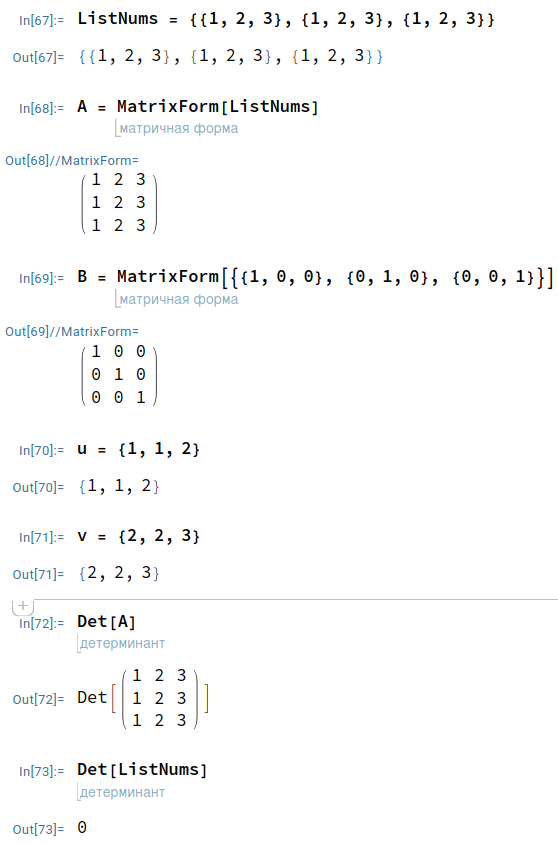
\includegraphics[scale=0.70]{body/img/7_1.png}}
    \label{fig:image_7_1}
\end{figure}

\begin{figure}[H]
    \renewcommand{\figurename}{Рисунок}
    \centering{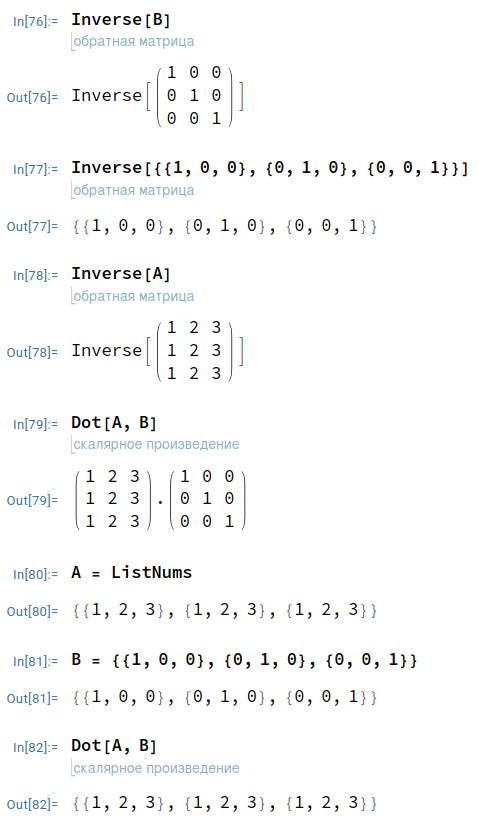
\includegraphics[scale=0.70]{body/img/7_2.png}}
    \label{fig:image_7_2}
\end{figure}

\begin{figure}[H]
    \renewcommand{\figurename}{Рисунок}
    \centering{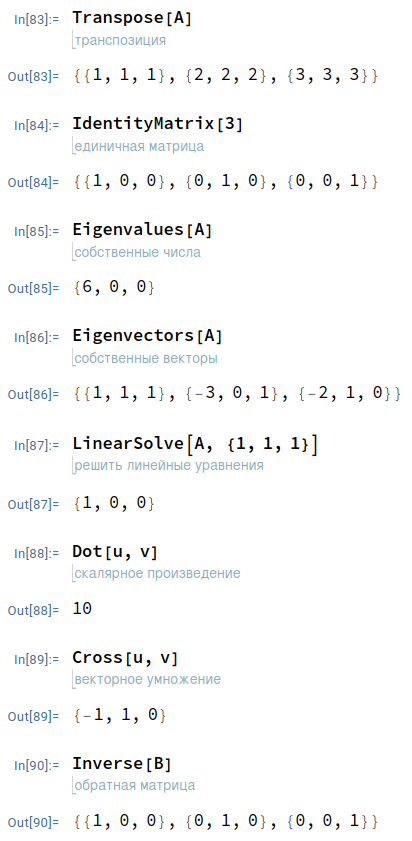
\includegraphics[scale=0.70]{body/img/7_3.png}}
    \label{fig:image_7_3}
\end{figure}